\chapter{Contribution process} \label{chapter6}
ACS UPB Mobile is hosted on GitHub\footnote{https://github.com/}, an internet solution for managing software versioning using Git\footnote{https://git-scm.com/}. As an open-source application, the project’s repository is open to everybody under the MIT license\footnote{https://opensource.org/licenses/MIT}, and this allows many developers to use or contribute to it.

~

For the purpose of this paper, we will explain how we adhered to the development process of the application using the tools provided by GitHub. We will present the steps involved, from proposing a feature to it being implemented, verified, and deployed. 

\section{Repository} \label{6:repo}
The ACS UPB Mobile repository is the main point of interest for us. Here we can find all the code versions, development guides, changelogs, and contact information. To ensure that any proposed feature is relevant to the application, the first step is to discuss with the project owner and reach an agreement about its implementation.
We can break this discussion for any features into three points that need to be clarified :
\begin{itemize}
            \setlength{\topsep}{0.5pt}
            \setlength{\itemsep}{0.5pt}
            \setlength{\parsep}{0.5pt}
            \item How it will affect the architecture and other components
            \item How it will affect the user interface and experience
            \item What opportunities for future features it enables
\end{itemize}

For the features proposed in this paper, we already answered these questions in the previous chapters. As this discussion was the first step in the implementation process, we had a clear development roadmap, as we knew ahead of time what challenges and opportunities each new feature provides. 

In order to keep track of the progress made, we created an issue inside the repository for each new feature. To further separate these related issues from the others, we also created a project for the general module.

This structure is illustrated in figure \ref{6:fig:planner} \footnote{https://github.com/student-hub/acs-upb-mobile/projects/6}.

\begin{figure}[ht]
    \centering
         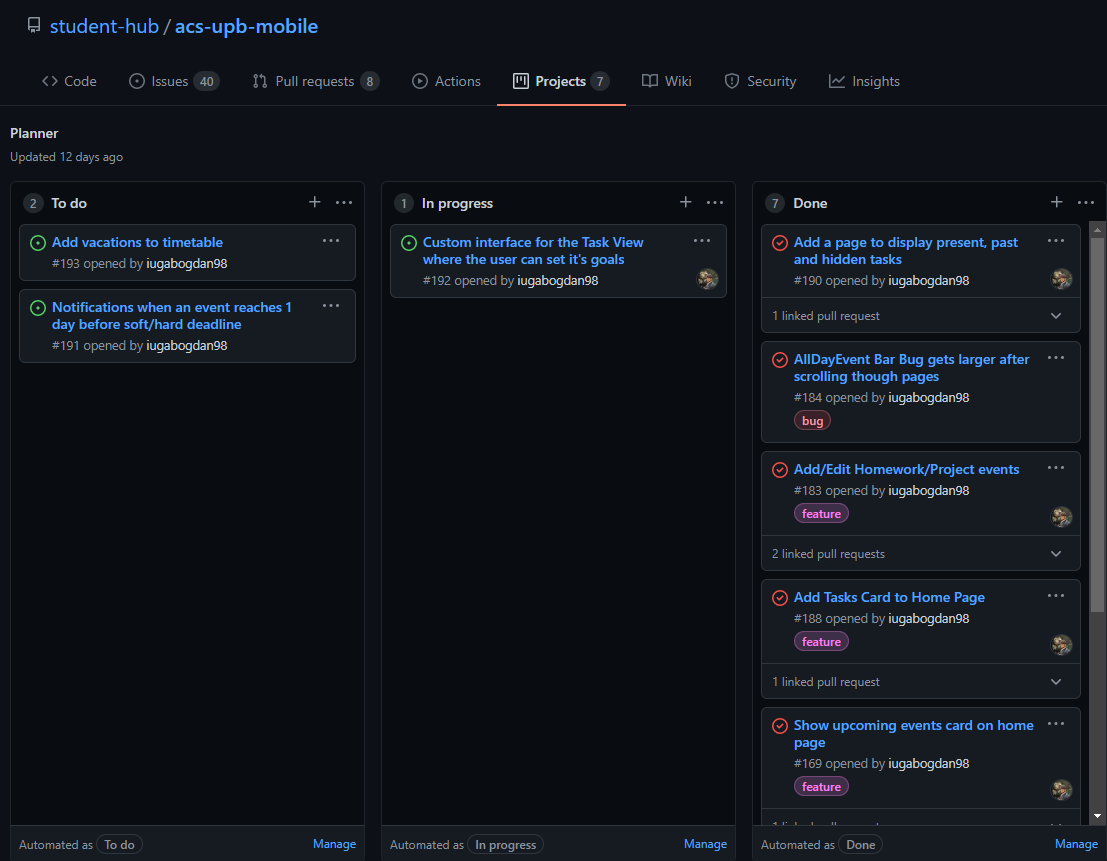
\includegraphics[width=0.95\textwidth]{figures/beforedev/image8.png}
    \caption{Planner project}  
    \label{6:fig:planner}
\end{figure}

~

Furthermore, because we were using Git, each of these issues had its own separate branch, meaning that the code was isolated while in development, assuring that we don’t change anything until the issue is resolved. 

\section{Pull Request} \label{6:pr}


When a feature is fully implemented, the next step is to add it to the project’s codebase, which is found on the “master” branch. As a security measure, merging code to the master branch has to meet a series of checks and approvals, and it is formally made by creating a pull request.

Before creating a pull request inside the application repository, we had to ensure that the following list of code quality checks is satisfied: 
\begin{itemize}
            \setlength{\topsep}{0.5pt}
            \setlength{\itemsep}{0.5pt}
            \setlength{\parsep}{0.5pt}
            \item The coding style corresponds to Dart standards.
            \item Dart analysis returns no warnings or errors.
            \item Each new text added is localized.
            \item All the automated tests are passed.
\end{itemize}

As some features may change the application, it is crucial that all the tests pass so that we know that even with a new feature, the application still behaves as intended. A concrete example of having to update the tests after developing a feature is that, when adding a new provider inside a page, it also has to be added in all the tests that use the page, otherwise they fail. In this way, we can check if the behavior of the new component produces a different result than the one expected. 
Github also automatically checks each pull request to ensure that the quality required is met.

The next step is requesting a code review, where in our case, the project owner manually checks the solution and decides if it is good to be merged. In the case of a negative response, further discussions happen where it is explained what is needed to be changed, and the process repeats until a positive response is given.

\section{Deployment} \label{6:deploy}


ACS UPB Mobile is, at the moment when this paper was written, available in the Google Play Store.

When a Pull request is approved and merged to the master branch, the code changes only in the repository. As we want to deliver these changes to the users, we need to deploy the application. This time of deployment and version number is established with the project owner and requires a list of changes that will be displayed to the users.

The deployment process is automated, and it is based on the tag mechanism used by Github. When pushing a new tag to the origin, the application is automatically deployed, and the code is checked automatically by the Play Store. When approved, it becomes available to the users. 


In the development process of the module proposed in this paper, we followed these steps and managed to deploy features that are now used inside the application. 

